\documentclass{article}
\usepackage{graphicx}
\graphicspath{ {./images/} }


% The preamble ends with the command \begin{document}
\begin{document} % All begin commands must be paired with an end command somewhere
\thispagestyle{plain}
    \begin{center}
        \Large
        \textbf{EC 0.6 - Reports}
        \\
        \vspace{0.4cm}
        \large
        \textbf{Alexander Razikov}
         \\
        \vspace{0.4cm}
        \large
        \textbf{CS 532, Spring 2023 }
         \\
        \vspace{0.4cm}
        \large
        \textbf{January 22, 2023}
    \end{center}
    
	%New section is created
	\section*{Q1}
	You may copy the question into your report, but make sure that you make it clear where the question ends and your answer begins.

	%New section about equations
	\subsection*{Answer}
	The example figure below shows the growth in the number of websites between 1993 and 1996.
    \\
    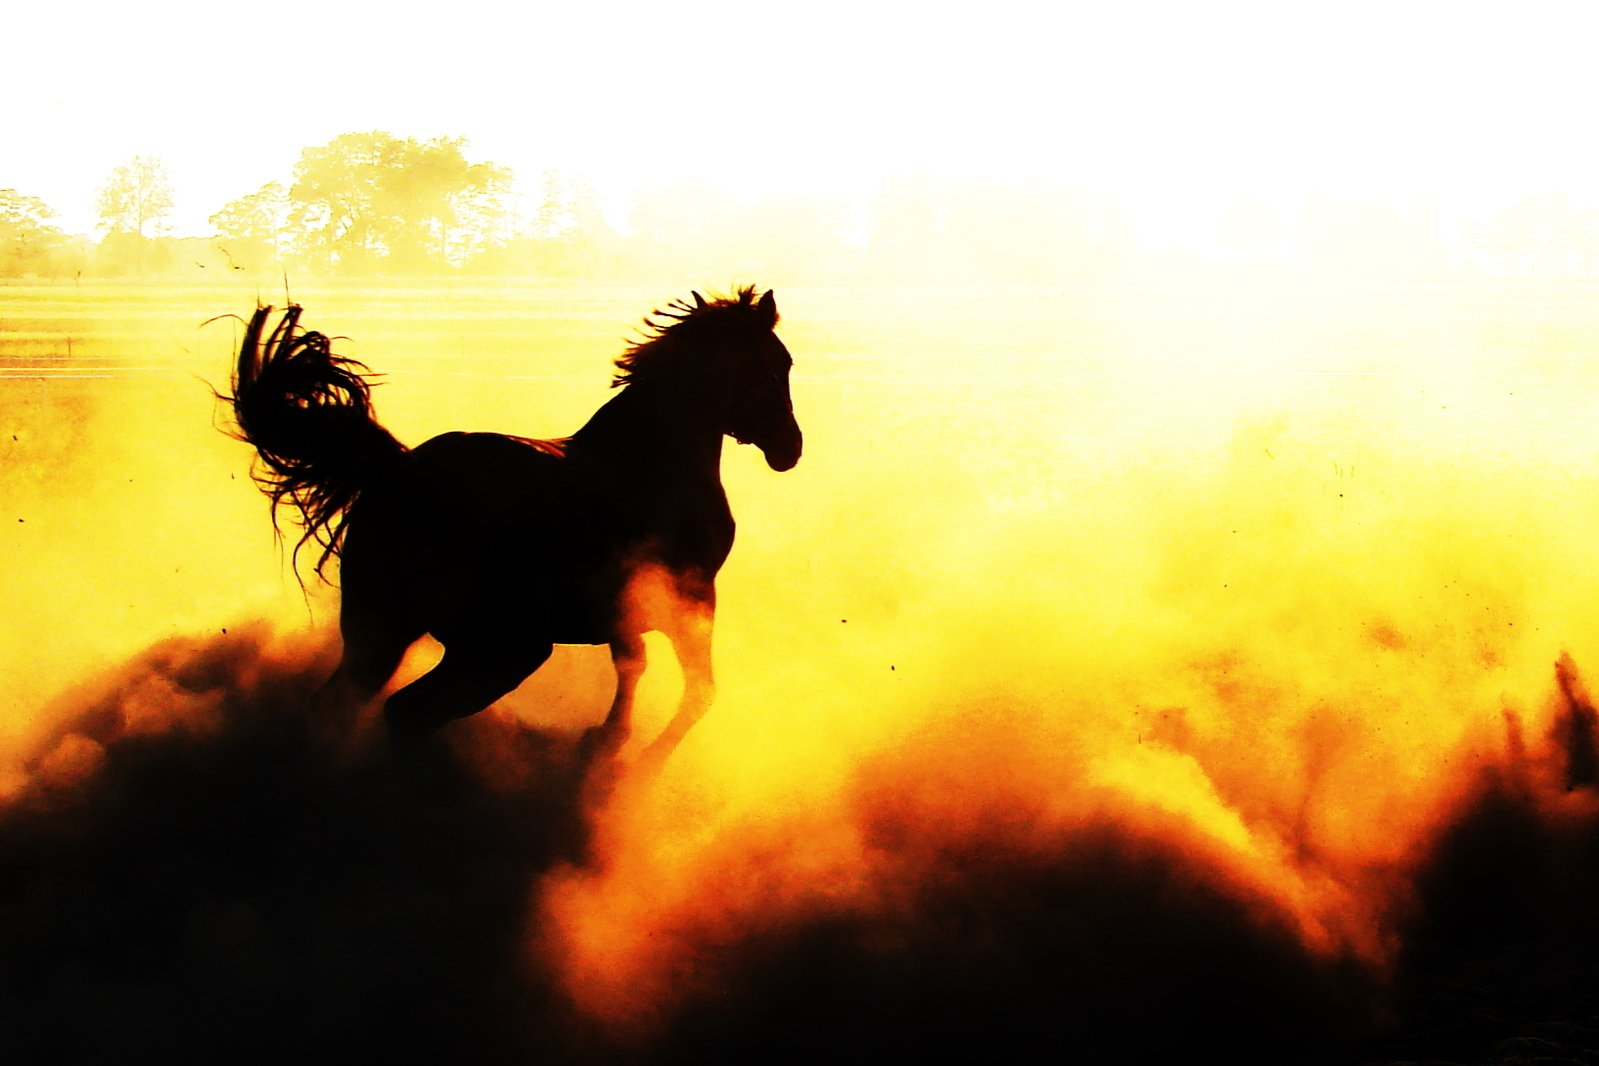
\includegraphics[scale=0.2]{images/horse.jpg}
    \\
    If you want to include code in your report, you can insert a screenshot (if it's legible), or you can copy/paste the code into a fenced code block.
    \begin{verbatim}
        import csv
        #read in the file
        with open("EC1\\friend-count.csv") as file:
        reader = csv.reader(file)
        counter=0
        #array for letters
        arr = []
        #array for totals   
        arrTwo=[] 
        #array for counts
        arrThree=[]
        for row in reader:
            if counter==0:
                counter= counter+1
            else:
    \end{verbatim}
	The table below shows a simple table.
\begin{table}[!ht]
    \centering
    \begin{tabular}{|l|l|l|}
    \hline
        Week & Week Start Date & Topic \\ \hline
        1 & Aug 27 & Introduction to Web Science and Web Architecture \\ \hline
        2 & Sep 3 & Introduction to Python \\ \hline
        3 & Sep 10 & Introduction to Info Vis with R, Python \\ \hline
        4 & Sep 17 & Measuring the Web \\ \hline
    \end{tabular}
\end{table}
\begin{abstract}
    The table below shows an example confusion matrix (you'll see this term later) from https://en.wikipedia.org/wiki/Confusion\_matrix. 
\end{abstract}
   

\begin{table}[!ht]
    \centering
    \begin{tabular}{|l|l|l|l|}
    \hline
        ~ & ~ & Actual & ~ \\ \hline
        **Predicted** & ~ & Cat & Dog \\ \hline
        ~ & Cat & 5 (TP) & 3 (FP) \\ \hline
        ~ & Dog & 2 (FN) & 3 (TN) \\ \hline
    \end{tabular}
\end{table}
	%New section about tables and figures
	\subsection*{Discussion}
 You must provide some discussion of every answer. Discuss how you arrived at the answer and the tools you used. Discuss the implications of your answer.

    \section*{Q2}
        \subsection*{Answer}
        \subsection*{Discussion}
    \section*{Q3}
        \subsection*{Answer}
        \subsection*{Discussion}
    \section*{References}
    Every report must list the references that you consulted while completing the assignment. If you consulted a webpage, you must include the URL.
    \begin{itemize}
        \item Overleaf, https://www.overleaf.com/learn/latex
        \item Python, https://docs.python.org/3/
        \item W3 Schools, https://www.w3schools.com/python/
        \item Horse Image, https://www.freeimages.com/photo/wild-horse-1334844
    \end{itemize}
\end{document} % This is the end of the document